\chapter{Gammel Kravspesifikasjon}
\label{chap:kravspesifikasjonGammel}
Kravspesifikasjonen gjelder for SSO løsningen prosjektet skal prosjektere. Ved behov gjelder også kravspesifikasjonen for eventuelle prototyper som lages for og bevise eller utdype ulike tekniske valg og løsninger.

\section{Hvordan kravspesifikasjon er utarbeidet}
\label{sec:kravspesifikasjonGammel_hvordanKravspesifikajsonErUtarbeidet}
Prosjektgruppen brukte et par uker på å sette seg inn i ulike autentiseringsløsninger før kravspesifikasjonen ble utarbeidet. Ingen på prosjektgruppen regnet seg selv om dyktige på fagområdet autentisering og autorisering av brukere, vi ga oss selv derfor en kort periode med faglig dypdykk før vi gikk i gang med utarbeidelse av en kravspesifikasjon for SSO løsningen Norkart ønsket.
\bigskip
Kravspesifikasjonen ble utarbeidet av prosjektgruppen på forespørsel fra product owner hos Norkart. Prosjektgruppen har jevnlig dialog med product owner for og sikre at oppgaven og kravspesifikasjon henger sammen.
\bigskip
I forhold til målbare data oppgitt i seksjon \ref{sec:kravspesifikajsonGammel_operasjonelleKrav} -  \nameref{sec:kravspesifikajson_operasjonelleKrav} på side \pageref{sec:kravspesifikajson_operasjonelleKrav} tok vi utgangspunkt i hva Norkart så for seg som et ekstremsenario for løsningen om de skulle selge svært mye og ha svært mye aktivitet. 

\section{Funksjonelle krav til løsningen}
\label{sec:kravspesifikajsonGammel_funksjonelleKrav}
Funksjonelle krav brukes for å si hva systemet skal utføre, og hvordan systemet skal reagere på ulike situasjoner. 

\subsection{Overordnet use case diagram}
\label{subsec:kravspesifikajsonGammel_funksjonelleKrav_overordnetUseCase}
For å beskrive hva endelig løsning skal inneholde av funksjonalitet og roller er det laget et overordnet Use Case (se figur \ref{fig:OverordnetUseCase-a} på side \pageref{fig:OverordnetUseCase}). Dette use caset er en skisse av Norkart ID som endelig løsning. For å begrense oppgaven ser vi for oss å fokusere på egenadministrasjon og innloggingsmekanismer. Dersom det blir tid til mer blir vi enig om hva som skal gjøres i samråd med Norkart. Nedenfor vil du kunne lese en kort forklaring av roller og funksjoner.

\begin{figure}[h]
    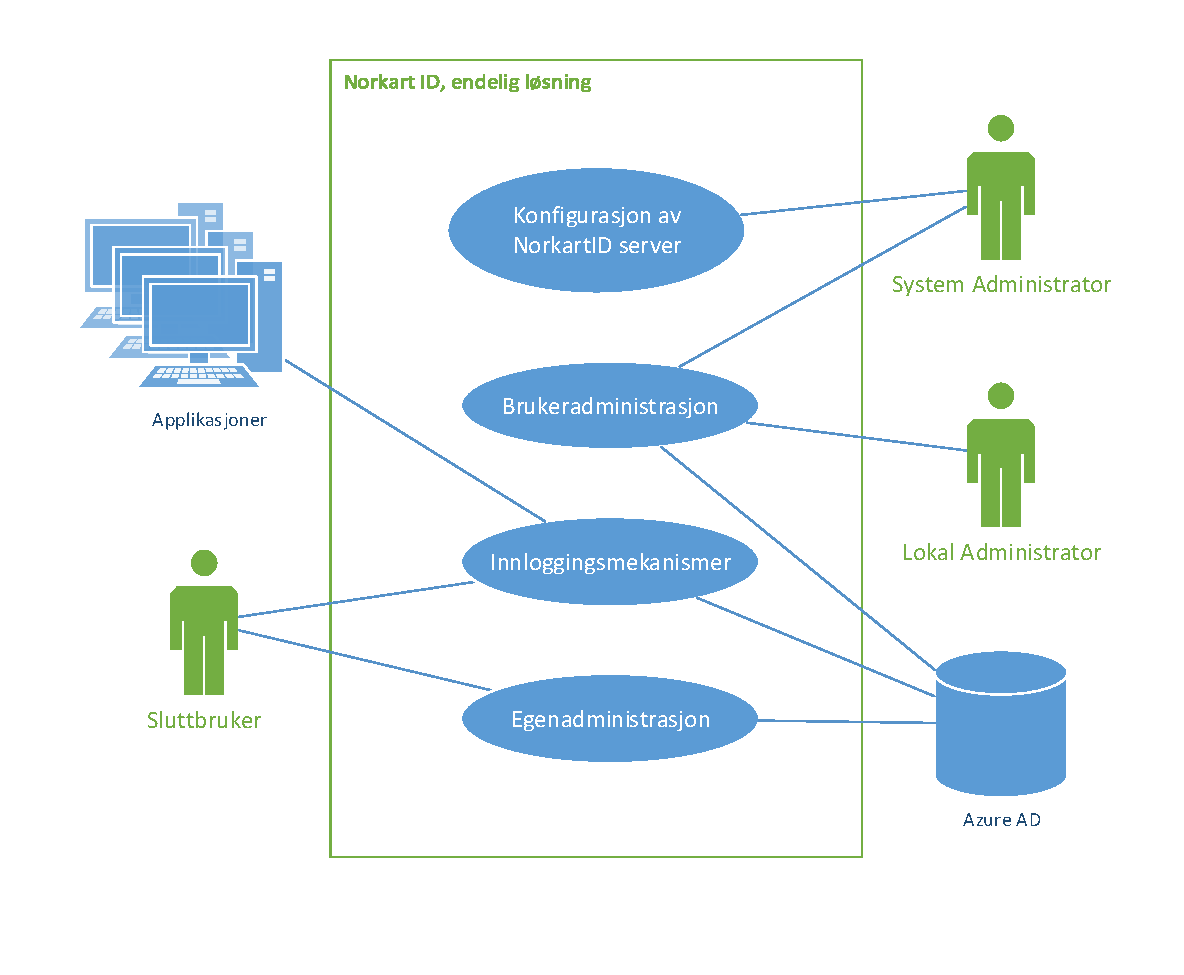
\includegraphics[scale=0.65]{graphics/OverordnetUseCase-a}
    \caption{Overordnet Use Case for endelig løsning av Norkart ID}
    \label{fig:OverordnetUseCase-a}
\end{figure}

\subsubsection*{System Administrator}
System administrator er rollen som setter opp hvordan Norkart ID systemet skal kobles sammen med applikasjonsserverene. System administrator har også mulighet til å administrere alle brukere som er tilkoblet systemet. 

\subsubsection*{Lokal Administrator}
Denne rollen har til hensikt å gjøre passordgjennoppretting og administrasjon av brukeretilgang tilgjengelig for bedriften som benytter seg av programvaren. Dette resulterer i redusert press på Norkart kundeservice. 

\subsubsection*{Azure AD}
Azure AD er brukerdatabasen Norkart ID skal benytte for å lagre brukerdata og tilgangsstyring. Den skal også kunne vedlikeholdes uten å gå via Norkart ID om dette er ønskelig. Ettersom all brukerdata lagres i Azure AD må alle roller som har mulighet til å endre brukerdata også kunne skrive eller oppdatere data igjennom Norkart ID. Azure AD brukes for å hente ut oppslag for hver eneste forespørsel om autentisering og autorisasjon av brukere mot applikasjoner.

\subsubsection* {Applikasjoner}
Applikasjoner er i dette tilfellet de applikasjonene Norkart ID skal autorisere brukere for å bruke. Norkart ID må kjenne til hvor og hvordan brukerne som autoriseres skal kontakte applikasjonene de er autoriserte for å bruke. Etter at en bruker logger seg inn med Norkart ID vil brukeren få informasjonsom trengs for å knytte seg til applikasjonene.

\subsubsection* {Sluttbruker}
Sluttbruker bruker Norkart ID som autentisering og autoriseringstjeneste. Dette er brukeren som logger inn med Norkart ID og får tilgang til tjenestene Norkart tilbyr.

\subsection {Use case diagram for prototype}
\label{subsec:prototype_use_case}
For å få et dypere innblikk av hva selve prototypen skal inneholde er det laget et use case diagram, se figur \ref{fig:PrototypeUseCase}, som inneholder roller og funskjoner basert på innloggingsmekanismer og egenadministrasjon i overordnet use case, se figur \ref{fig:OverordnetUseCase}. Innlogggingsmekanismer er her delt opp i tre funksjoner og e-post er tatt med som eksternt system. 

\begin{figure}[h]
    \includegraphics[scale=0.65]{graphics/PrototypeUseCase}
    \caption{Use Case Diagram for prototypen av Norkart ID }
    \label{fig:PrototypeUseCase}
\end{figure}

\subsubsection* {Applikasjoner}
For at bruker skal kunne logges inn må Norkart ID vite hvilken applikasjon bruker vil logge inn på. Derfor trenger rollen applikasjoner, se figur  \ref{fig:PrototypeUseCase}, kun tilgang til logg inn funksjonalitet.

\subsubsection* {Sluttbruker}
Sluttbruker kan benytte all funksjonalitet i prototypen.

\subsubsection*{Azure AD}
Ettersom bruker må autentiseres for å logge inn og ut og bruke glemt passord funksjonalitet  må Norkart ID ha tilgang til Azure AD for å utføre disse funskjonene. Norkart ID må også ha tilgang til Azure Ad for å endre brukerdata under egenadministrasjon.

\subsubsection* {E-post}
For at Norkart ID skal kunne gjennomføre glemt passord funksjonalitet trenger den tilgang til en E-post server. Hvis en bruker har glemt passord skal Norkart ID sende en resett passord link på e-post til brukeren.

\subsection{Høynivå use case beskrivelser}
\label{subsec:kravspesifikasjonGammel_funksjonelleKrav_hoyNivaa}
4 høynivå use case beskrivelser er definert for å beskrive funksjonalitet i løsningen.

\begin{framed}
    \begin{tabular}{l p{9cm}}
        \textbf{Use case:} & Logg inn \\
        \textbf{Aktører:} & Sluttbruker, Applikasjon og Azure AD \\
        \textbf{Mål:} & Bruker skal kunne få tilgang til ønsket applikasjon. Applikasjon skal være sikker på at bruker har tilgang \\
        \textbf{Beskrivelse:} & Når bruker skriver inn brukernavn og passord skal brukeren autentiseres og få tilgang til applikasjonen den ønsker å jobbe på.
    \end{tabular}
\end{framed}
\begin{framed}
    \begin{tabular}{l p{9cm}}
        \textbf{Use case:} & Logg ut \\
        \textbf{Aktører:} & Sluttbruker og Azure AD \\
        \textbf{Mål:} & Bruker skal kunne få logget ut av ønsket applikasjon og fra alle andre tjenester \\
        \textbf{Beskrivelse:} &  Når bruker klikker logg ut skal brukeren bli utlogget i alle systemet, både web, mobil og applikasjonsnivå. En singel-sign-out(for aktivt token) måte hvor man slipper å måtte logge ut individuelt i alle systemer.
    \end{tabular}
\end{framed}
\begin{framed}
    \begin{tabular}{l p{9cm}}
        \textbf{Use case:} & Glemt passord \\
        \textbf{Aktører:} & Sluttbruker, Azure AD og E-post \\
        \textbf{Mål:} & Bruker skal kunne få mulighet sette nytt passord og få logget inn igjen. \\
        \textbf{Beskrivelse:} &  Bruker skal kunne hente ut passord selv til sin brukerprofil uten å måtte kontakte kundeservice. Her er tanken at man skal kunne motta en epost med en reset link hvor du kommer inn direkte til hvor du skal opprette nytt passord.
    \end{tabular}
\end{framed}
\begin{framed}
    \begin{tabular}{l p{9cm}}
        \textbf{Use case:} & Egenadministrasjon \\
        \textbf{Aktører:} & Sluttbruker og Azure AD \\
        \textbf{Mål:} &  Bruker skal kunne endre på registrerte opplysning inne på sin brukerprofil. \\
        \textbf{Beskrivelse:} &  Når bruker er autentisert skal han kunne gå inn for å endre på sin profil. Det er her sluttbruker får tilgang til epost, telefon, generelle opplysning som er registrert. Brukeren har her mulighet til å endre de attributtene som går an og endre. Dette er en egen nettside hvor bruker får tilgang til etter autentisering.
    \end{tabular}
\end{framed}

\subsection{User Stories}
\label{subsec:kravspesifikasjonGammel_funksjonelleKrav_userStories}
For å få en dypere forståelse av hva slags funksjonalitet som trengs for å overholde kravene til oppgaven har vi utarbeidet user stories som viser hva de forskjellige brukerne av applikasjonen skal kunne å utføre. De er utarbeidet ut fra use case diagram for prototypen, (se figur \ref{fig:PrototypeUseCase} på side \pageref{fig:PrototypeUseCase}), og oppgavens operasjonelle krav (se seksjon \ref{sec:kravspesifikajson_operasjonelleKrav}).


\section{Operasjonelle krav til løsning}
\label{sec:kravspesifikasjonGammel_operasjonelleKrav}
Operasjonelle krav brukes for å beskrive kvaliteten på systemet, dette kan være i form av standarder som benyttes, målinger som skal være innenfor en gitt grense og kostnadder.

\subsection{Ytelse}
\label{subsec:kravspesifikasjonGammel_operasjonelleKrav_ytelse}
\begin{itemize}
\item Løsningen skal som minimum takle 10 000 brukere innlogget samtidig.
\item Løsningen skal håndtere pålogging av 100 brukere i minuttet.
\item Løsningen skal bygges for å være skalerbar.
\item Det skal ta mindre enn et sekund å autentisere en bruker for de systemene brukeren er autorisert for å bruke.
\item Om belastning på NorkartID serversystemet skulle bli så høy at overordnede krav til innloggingstid ikke overholdes vil operasjoner og forespørsler fra brukere behandles etter FIFO-kø prinsippet.
\end{itemize}

\subsection{Implementasjon}
\label{subsec:kravspesifikasjonGammel_operasjonelleKrav_implementasjon}
\begin{itemize}
\item NorkartID skal fungere som en autentiserings- og autoriseringsledd mellom brukerne og tjenestene Norkart tilbyr.
\item Løsningen skal kjøres på en Microsoft Windows server 2012 eller nyere.
\item Løsningen skal benytte Azure AD brukerdatabase.
\item Innloggingsløsningen skal baseres på OpenID Connect biblioteker.
\item NorkartID skal designes for eksterne brukere.
\end{itemize}

\subsection{Standarder}
\label{subsec:kravspesifikasjonGammel_operasjonelleKrav_standarder}
\begin{itemize}
\item Løsningen skal tilfredstille kravene til OpenID Connect standardene.
\item Løsningen skal igjennom bruk av OpenID Connect tilfredstille sikkerhetsmekanismene gitt ved å burke OAuth 2.0
\item All kommentering og dokumentasjon av kildekode skal gjøres i henhold til normer gitt for programeringsspråkene som brukes i prosjektet.
\end{itemize}

\subsection{Pålitelighet}
\label{subsec:kravspesifikasjonGammel_operasjonelleKrav_pålitelighet}
\begin{itemize}
\item Pålitelighet i forhold til oppetid av Azure plattformen medregnes ikke i dette prosjektet. 
\item Azure AD skal håndteres slik at den aldri skal trenge å taes ned. 
\item Systemet skal designes for å ha en oppetid på minimum 99,9 \%, det vil si 10 minutter nedetid for vedlikehold i uken.
\item NorkartID serveren, Open ID Connect og Azure AD skal kunne vedlikeholdes individuelt.
\item Systemet stiller ingen krav til å kunne oppdateres mens det kjører.
\item Kundestøtte for NorkartID vil implementeres hos eksisterende kundeservice.
\end{itemize}

\subsection{Brukervennlighet}
\label{subsec:kravspesifikasjonGammel_operasjonelleKrav_brukervennlighet}
\begin{itemize}
\item Løsningen skal følge regler for universell utforming (se lover og regler)
\item Bruker skal kunne bruke samme påloggingsinformasjon mot alle systemene til Norkart.
\item Brukere skal selv kunne administrere brukerprofil og passord
\item Brukergrensesnittet skal være så intuitivt at det tar mindre enn 2 sekunder å skjønne hvor brukerid felt, passord felt og innloggingsknappen er.
\item Brukergrensesnittet på løsningen skal være skrevet på norsk.
\item Brukergrensesnittets design skal skape gjenkjennelighet til Norkart.
\item Fremdriftsindikator skal brukes der det er hensiktsmessig for å gi brukeren tilbakemelding.
\item Når bruker lager passord skal det gis indikasjon på om passordkravene tilfredstilles.
\end{itemize}

\subsection{Lover og regler}
\label{subsec:kravspesifikasjonGammel_operasjonelleKrav_lover_regler}
\begin{itemize}
\item Systemet skal håndtere data i samsvar med lov for Norsk personvern
\item Systemet skal følge forskrift om universell utforming av informasjons- og kommunikasjonsteknologiske (IKT)-løsninger
\end{itemize}

\subsection{Intraoperabilitet}
\label{subsec:kravspesifikasjonGammel_operasjonelleKrav_intraoperabilitet}
\begin{itemize}
\item Systemets API skal kunne kommunisere over standard http protokoll.
\item Systemets API skal støtte autentisering, glemt passord funksjonalitet og fornying av økt.
\item Brukergrensesnitt på løsningen skal være responsivt.
\item Systemet skal ha støtte for Single Sign On på Microsoft Windows 8 (eller nyere windows systemer).
\end{itemize}

\subsection{Sikkerhet og autentiseringskrav}
\label{subsec:kravspesifikasjonGammel_operasjonelleKrav_sikkerhet}

\begin{itemize}
\item Brukerdata løsningen trenger: Fullt navn, selskap, mail, passord, mobil, sist innlogget og gjeldende autentiserte enheter. 
\item All lagring av brukerdata skal beskyttes i forhold til trusselbilde. 
\item Ingen passord skal sendes eller lagres i klartekst.
\item Systemet skal følge generelle normer innenfor autentisering
\item Minimumskrav for passordlengde er 8 tegn.
\item Minimumskrav for passordkompleksitet er minimum en stor og en liten bokstav, og minimum et tall. 
\item Etter 5 feilede innloggingsforsøk mot en bruker id skal det legges inn ventetid på 1 minutt før det tillattes nytt innloggingsforsøk mot samme bruker id.
\item Ved feil passord eller brukernavn skal det kun stå at innlogging feilet. 
\item Ved glemt passord skal det sendes link til bruker for generering av nytt passord. Denne linken skal kun være gyldig i 20 minutter.
\item En sesjon er kun gyldig 6 timer før den må fornyes.
\item En bruker som logger inn via en nettleser  autentiseres for alle web applikasjoner brukeren har tilgang til i den nettleseren.
\item En bruker som logger inn i en mobil applikasjon autentiserers kun til denne applikasjonen
\item En bruker som logger inn i en desktop applikasjon autentiseres kun til denne applikasjonen.
\end{itemize}

\subsection{Klientkrav}
\label{subsec:kravspesifikasjonGammel_operasjonelleKrav_klientkrav}
\begin{itemize}
\item Det kreves at klienten har tilgang på en nettleser som leser HTML5, CSS3 og JavaScript.
\item Klienten må gi tilgang til cookies for å bruke Single Sign On funksjonaliteten i nettleser.
\item Klienten må ha skriverettigheter i maskinens register for å bruke Single Sign On funksjonaliteten på skrivebordsapplikasjoner.
\item Det kreves at klienten er tilkoblet internett eller i nettverk med NorkartID serveren.
\item Det kreves at klienten har nettverkshastighet tilsvarende 0,4 Mbit eller høyere for garantert stabil tilkobling til tjenesten (stabil Edge eller høyere tilkobling).
\end{itemize}


\section{Krav til resultat av prosjektoppgaven}
\label{sec:kravspesifikasjonGammel_kravTilResultatAvProsjektoppgaven}
{\color{red}TODO}\\
Oppgaven skal skrives etter regningslinjer gitt for bachelor og masteroppgaver ved Høyskolen i Gjøvik.
\\
\\
\href{http://www.hig.no/content/download/30554/364363/file/Retningslinjer%20for%20mastergradsoppgaver%20og%20st%C3%B8rre%20studentoppgaver%20p%C3%A5%20bachelorniv%C3%A5%20ved%20H%C3%B8gskolen%20i%20Gj%C3%B8vik_des2010_v1201.pdf}{Link til retingslinjene}

